\part{Data \& Methods\label{cha:datamethods}}

%%%%%%%%%%%%%%%%%%%%%%%%%%%%%%%%%%%%%%%%%%%%%%%%%%%%%
  
\chapter{Data\label{cha:Data}}

  In the present chapter, the databases used in the manuscript are described. Different types of data are used in each of the studies due to the fact that different problems are addressed. A more specific description is included in later chapters.\\

  There are many applications from meteorology to agriculture or even health sciences, that would benefit from an accuarate station network that provide high quality radiation measurements at the surface. However, it is well-known that the lack of  well spread solar radiation measurements has been a constrain not only for the development of solar forecasting or resource assessment techniques, but also for the study of the whole atmospheric/climatic processes in which solar radiation takes places. The progress and improvement in the satellite-based products has helped to overcome some of these issues providing gridded data at a high spatial and temporal resolution.\\

  \section{Solar radiation measurements: \textit{Baseline Surface Radiation Network, BSRN}}

  Solar radiation data from ground stations are not common at the publicly available metheorological stations. One of the main sources of high quality data are from the 'Baseline Surface Radiation Network', BSRN \cite*{Konig-Langlo2013}.\\ %[König-Langlo, G. , Sieger, R. , Schmithüsen, H. , Bücker, A. , Richter, F. and Dutton E.G. 2013. The Baseline Surface Radiation Network and its World Radiation Monitoring Centre at the Alfred Wegener Institute.
%GCOS - 174, WCRP Report 24/2013, 30 pp..] \\

  The aim of the BSRN project is to detect changes in the Earth's radiation field that could be a consequence of climatic changes [ref web]. The monitoring network provides high-quality and high-frequence data of short and long-wave radiation fluxes from different stations around the globe, which correspond to different climatic zones. In figure \ref{fig:bsrnstations} all the available stations from BSRN are displayed.\\

The World Climate Research Programme (WCRP) Radiative Fluxes Working Group initiated the Baseline Surface Radiation Network (BSRN) to support the research projects of the WCRP and other scientific programs related to solar radiation. By the time this manuscript is written, 52 BSRN are in operation. There are some stations with 'candidate' status and some that will be close in 2019. Among these stations there are different levels of data provided, from the basic measurements that include the components of solar radiation, air temperature and pressure to other variables and synoptic observations.

\begin{figure}[h]
  \centering
  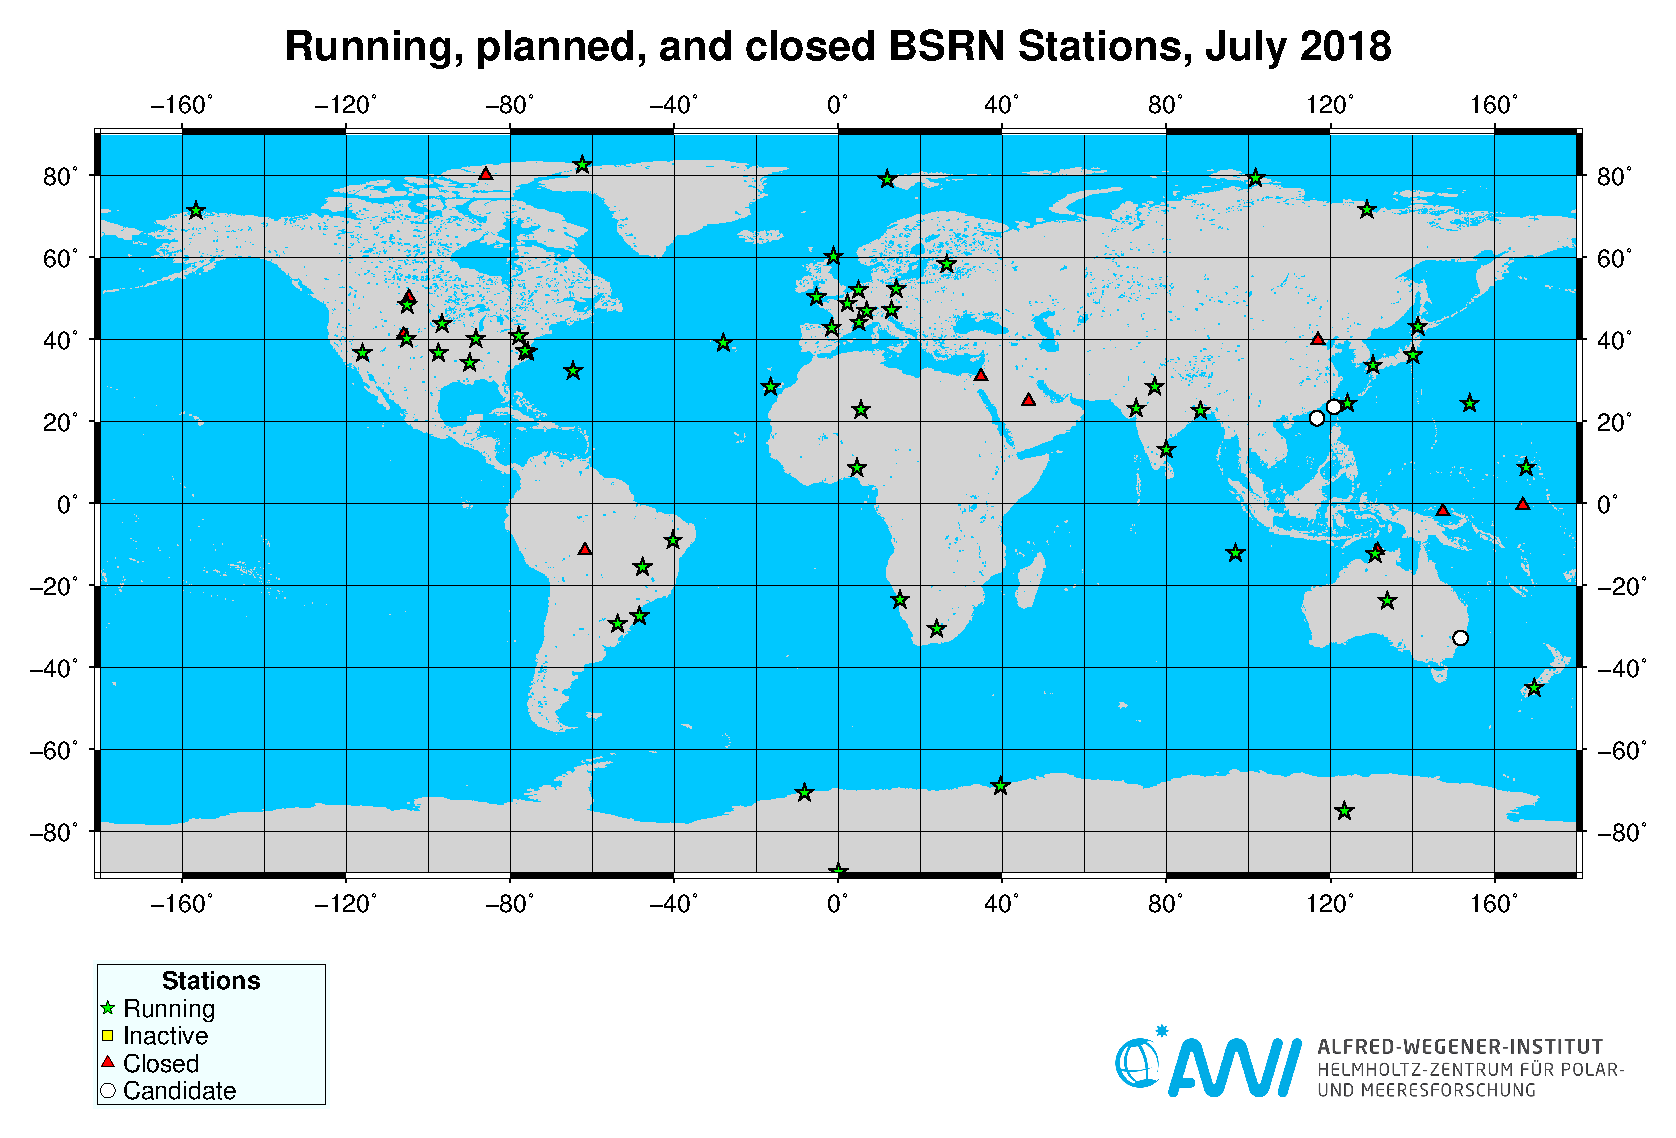
\includegraphics[width=0.8\textwidth]{DataMethodsFIGS/bsrn.pdf}
  \caption{Solar radiation stations from BSRN.}
 \label{fig:bsrnstations}
\end{figure}

\section{Modelling of solar radiation}

In order to understand the processes that take places when solar radiation goes through the atmosphere and reaches the Earth's surface it is necessary a modelling approach. This modelling process can be made by a physical approach or using statistical methods (Festa and Ratto, 1993).\\

The physical modeling of solar radiation is based on physical equations of the interaction between atmospheric components and solar radiation (aerosols, water vapour, clouds...). When solar radiation goes through the atmosphere, it can interact with its components being absorbed by molecules, backscattered to space or scattered in any other direction. Thus, only part of the solar radiation at the top of the atmosphere (TOA) will reach the Earth's surface.\\ 

This process is the physical process of energy transfer described by the radiative transfer equation (RTE) and its solution needs a radiative transfer model (RTM). The radiative transfer is a very complex process that needs to be simplified to be solved numerically and some parametrizations are needed. However, from these models it is possible to reproduce the solar radiation behaviour across the atmosphere and at the surface. RTMs are in the core of numerical weather prediction models and climate models and sometimes they are used to obtain solar radiation from satellite images, although in this case empirical or semi-empirical approaches are also commonly applied.\\

Secondly, the solar radiation at the surface can be estimated using statistical methods. In this case it is necessary to have enough data to validate the model and likely these models will not be able to reproduce solar behaviour universally. However, they can be very useful for local applications.\\

In chapters 6 and 7 different climate models are used as main source of solar radiation data. The output of each model will be the result of the radiative scheme inside their codes and it can be used as the input variable for a photovoltaic production model to analyse photovoltaic potential under different climate conditions.\\

\subsection{CORDEX initiative}

Under the acronim of CORDEX (Coordinated Regional Downscalling Experiment) there have been developed a wide range of regional climate models\footnote{The chapter \ref{cha:Methods} explain the origin of regional climate modelling and the simulations used in the thesis} that provide climate downscalled simulations for different areas around the globe\footnote{Cordex website:http://www.cordex.org/. This international framework is under the umbrella of the world climate research program, WRCP} . Their importance arise with the advance in knowdlege of climate change provided by global models. Whereas those models give an overview of the evolution of global conditions, their coarse resolution is not enough to understand climate change impacts at a local scale. The higher resolution of the regional climate models are needed for supporting adaptation and mitigation plans.\\

Two different domains from CORDEX are used in this study both focus on the Mediterranean area: EURO-CORDEX and MED-CORDEX (in figure \ref{fig:cordexdomain}). The horizontal resolution of the simulations included in EURO/MED-CORDEX go from 44º to 11º (from ~50km to ~12km).

\begin{figure}[!tbp]
  \centering
  \subfloat[Med-CORDEX]{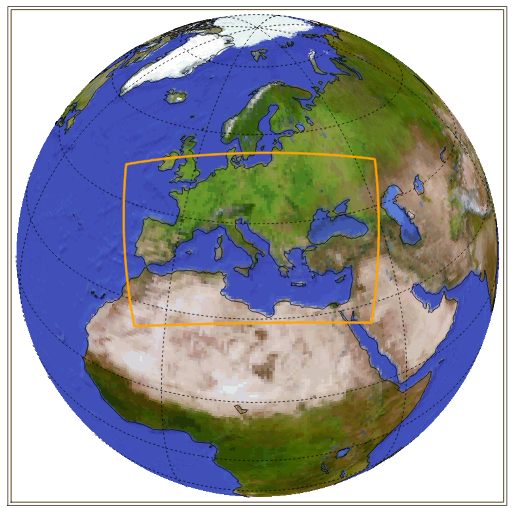
\includegraphics[width=0.4\textwidth]{DataMethodsFIGS/medcordex2}\label{fig:medcordex}}
  \hfill
  \subfloat[Euro-CORDEX]{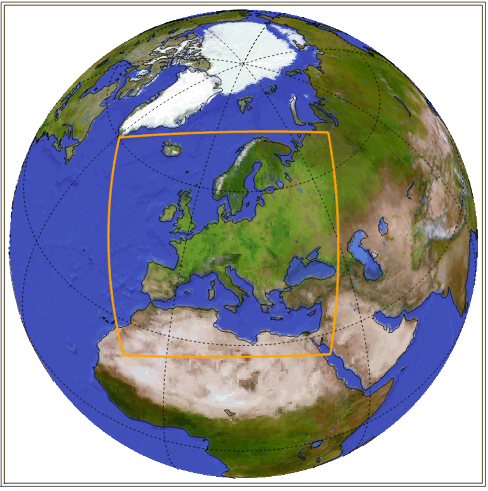
\includegraphics[width=0.4\textwidth]{DataMethodsFIGS/eurocordex2}\label{fig:eurocordex}}
  \caption{Domains from Med-CORDEX and Euro-CORDEX. Images from wRCP-CORDEX website.}
    \label{fig:cordexdomain}
\end{figure}

{\color{red}¿Incluir una tabla con los diferentes modelos regionales que participan en MED cordex y EURO cordex? Los que se usan en la tesis están explicados después, pero este es un punto general de dónde se han obtenido los datos.}
\section{Satellite data: \textit{Climate Monitoring Satellite Application Facility, CM-SAF}}

It has been previously commented that the scarcity of available ground-based solar radiation measurements is a well-known problem. Satellite datasets have become one of the main sources of solar radition data because of their high spatial and temporal resolution as well as their increasing accuracy.\\

There are different methods to retrieve solar radiation from satellite images that goes from physical models to empirical ones. In the first case, the models try to explain the radiance observed by the satellite instrumentation with a radiation transfer model (RTM). In order to do that, it is necessary to know the composition of the atmosphere. On the other hand, empirical models are based in simple regression models between the visible-channel's recorded intensity and grounded measurements. There are also some approaches that are in between theses two sides: the semi-empirical models. They use a simpler radiative-transfer scheme and some statistical regressions between data from satellite sensors and observed data (Schmetz (1989), Noia et al. (1993), Pinker et al. (1995), Zelenka (2001), and Hammer et al (2003)).\footnote{Jan Kleiss, Solar Energy Forecasting and Resource assessment, pp.22.23}\\

In this work some satellite-data-based products from CM-SAF (The Satellite Application Facility on Climate Monitoring) have been used. The aim of CM-SAF consortium from EUMETSAT [ref] is to develop satellite-data-based-products for climate monitoring since in 2000 it was recognised the importance of using satellite for this purpose.\\

The CM SAF products are derived from several instruments on-board operational satellites in geostationary and polar orbits. There are two main types of products that can be obtained from the CM-SAF: operational products and climate data records (CDR). The main purpose of the CDR is to provide a high-quality database to monitor climate variability and changes (ref), as well as the detection of trends. Operational products, on the other hand, are not accurate enough for this purpose because some errors like inter-satellite biases or sensors degradation are not corrected (ref: PUM producte user manual).\\


The SARAH dataset from CM-SAF has been used in chapters 6 and 7 of this manuscript for the analysis of shortwave solar radiation at the surface. The data is based on the records from Meteosat images, first and second generation, using the on-board MVIRI and SEVIRI instruments respectively. As the purpose of the CDR is to provide long time series convering more than 20 years, it is necessary a retrieval algorithm that can be applied to SEVIRI intruments as well as to the older MVIRI. This algorithm has been called MAGICSOL and has to parts: first, the modified Heliosat method is used to obtain the cloud effective albedo (CAL) and second, the MAGIC appoach is used to obtain all sky surface radiation based on CAL. (ref PUM)\\

{\color{red} No sé si merece la pena poner algo más acerca del método. Puede ser de ayuda también para ver como se incluyen los aerosoles. Incluyo una imagen del esquema que hice del proceso de obtención de la radiación con los datos del satélite y podría estar bien incluir.}\\


\begin{figure}
  \centering
  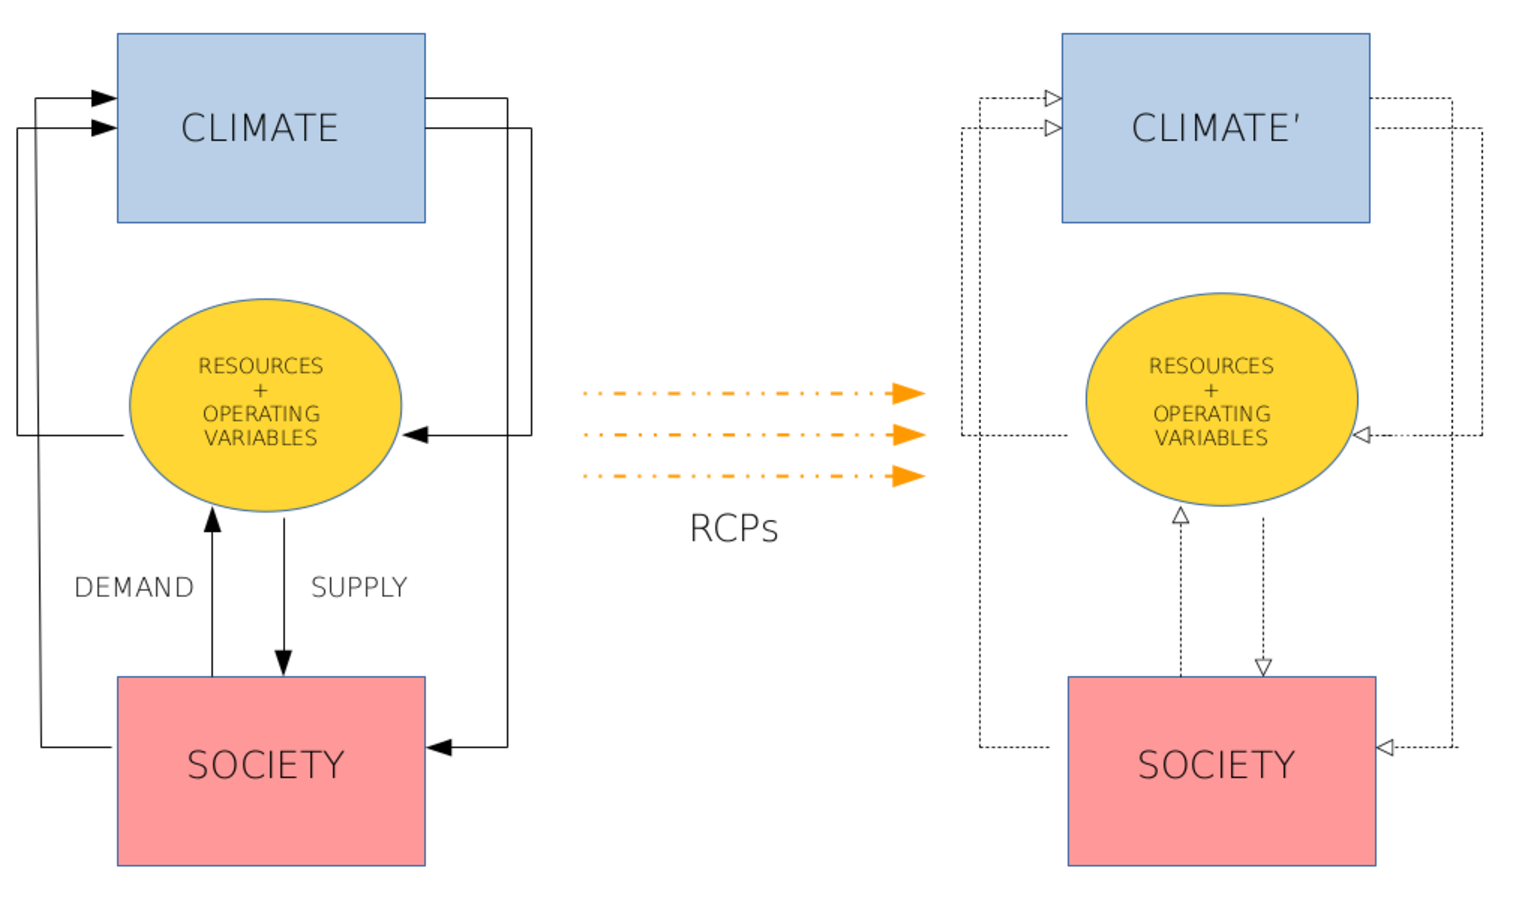
\includegraphics[width=0.6\textwidth]{figs/esquema}
  \caption{Algorithm scheme: Retrieval of shortwave solar radiation from satellite images.}
 \label{fig:algorithm}
\end{figure}

\section{Photovoltaic prodution data}

In order to evaulate the performance of a PV model it is necessary to use the data from real PV plants. However, these data is not easy to obtain, due to the fact that it belongs to private companies and it could compromise some of their strategies. This makes necessary to get agreements and confidential contracts between these companies and researchers that are not always easy to obtain if an inmediate benefit does not arise from those relationships.\\

Some alternatives are the databases of aggregated data that are available for the European countries throught the ETNSO-e data portal website. However, these data will be only useful for certain modeling exercices.\\

\begin{itemize}
\item {\color{red} ¿Tiene sentido que comente aquí los datos de ETNSO?}
\item {\color{red}No tengo claro si describir aquí las dos plantas que tenemos y que se utilizan en el segundo artículo}\\
\end{itemize}

\section{Temperature data}

  In adittion to the direct relationship between solar irradiation and photovoltaic energy conversion, there are other atmospheric variables that influence the performance of solar cells, like temperatura or wind speed. The model used in this work consider only temperature as a second order factor that reduces cell efficiency as it is explained in chapter 4.\\
 
  Temperature data is easier to obtain than solar radiation data. Numerous weather stations provides temperature data at 2m over the surface at a local scale. For an overview of a large area gridded products are useful and easier to combine with the satellite products.\\

  E-OBS is a gridded dataset derived through interpolation from the ECA\&D data based on stations that provides daily temperatura data over Europe and the Mediterranean area \footnote{https://www.ecad.eu//download/ensembles/download.php#maps}. This product has been validated in several research papers (Begert et al. 2008, Hofstra et al. 2009a,b) finding that some inaccuaracies related to an over-smooth exists in areas where there are few stations, which affects mostly to the extreme analyses.

{\color{red} ¿Quizás incluir aquí un mapa con las estaciones a partir de las que se hace la interpolación}  
%%%%%%%%%%%%%%%%%%%%%%%%%%%%%%%%%%%%%%%%%%%%%%%%%%%%%
\chapter{Methods\label{cha:methods}}

In order to fullfill the objectives of the present work it is necessary to apply different methodologies in each of the results chapters, all of them has been explained in detail at the corresponding section.\\ %In general, they goes through the statistic analysis of different variables related to solar resource and photovoltaic production, where the latter comes from an estimation using a PV model. %The analysis is also developed in different time scales, which leads to the necessity of adapt the same methodology to each case.\\

However, in the present chapter the different tools needed for the development of each study are described in a general manner. The three results chapters are based in a \textbf{modeling chain} that includes a photovoltaic model that is composed of two basic steps. First, the transposition to the plane-of-the-array, POA, of the components of the solar radiation, which implies also to assume some simple models of the atmosphere sphere seen from the generator plane and a model for the electrical performance of the system. Besides, the input of this PV model can be solar radiation measurments, satellite radition estimations o, as we saw in the previous chapter, the output of atmospheric/climate models. \\

%En general, el método consite en la creación de una cadena de modelado que incluye un modelo de producción fotovoltaica, compuesto por el paso al plano del generador fotovoltaico de las componentes de la radiación solar y un modelo de funcionamiento eléctrico del sistema. Además, se el input de este modelo fotovoltaico podrán ser observaciones de radiación solar medidas en superficie, estimaciones de satélite o, como vimos en el capítulo anterior, radiación solar obtenida a partir de la salida de modelos.
%  En el primer capítulo, se analizará de manera espacial la variabilidad interanual y la complementariedad del recurso solar en la Península Ibérica, para lo que se aplicarán técnicas de \textbf{clustering}. La evaluación de la productividad fotovoltaica lleva asociada la necesidad de la \textbf{modelización de un sistema fotovoltaico}.\\

  In chapter 5 it is analysed the interannual variability and complementarity of solar resource over the Iberian Peninsula and for that purpose we apply \textbf{clustering techniques}. The regionalization allow us to simplify the spatio-temporal analysis of solar resource. The evaluation of the productivity, defined as the amount of energy produced by a PV system normalized by the power capacity of the system, means the \textbf{modelization of the photovoltaic system}.\\
  
  The chapter 6 analyses the impact of \textbf{aerosols} in photovoltaic productivity over the Euro-Mediterranean area.  Some climate simulations are used as the input of the photovoltaic model. The modelling chain allows to make a sensitivity test to quantify the role of aerosols in the area.\\

%  En el segundo capítulo se estudia el impacto de los aerosoles en la producitvidad fotovoltaica, esta vez en el área Euro-Mediterránea. En este caso, las \textbf{simulaciones climáticas} serán utilizadas como input del modelo fotovoltaico, creando una cadena de modelado que permita realizar un ejercicio comparativo de sensibilidad para cuantificar el papel de los aerosoles.\\
  
  Finally, the photovoltaic energy potential is analysed in the future, using \textbf{climate projections} from different climate models. Trends and anomalies with respect to a reference period are evaluated. In this case, a \textbf{multi-model analysis} through different RCMs simulations allow us to evaluate the solar resource under climate change scenarios. The representation of aerosols in the climate projections is consider as a fundamental variable for the shortwave downward radiation projections, SSR, and PV productivity.\\ 

%  Por último, se realiza el análisis del potencial fotovoltaico futuro, evaluando las tendencias y anomalías con respecto a un periodo de referencia. En este caso, se hace un \textbf{estudio multimodelo} a través de distintas simulaciones de diferentes RCMs que permita evaluar el recurso solar y se utilizan las mismas para el cálculo de la producción fotovoltaica. En este último punto vuelve a considerarse la representación del campo de AOD dentro de las simulaciones climáticas como variable determinante en las proyecciones de SSR y productividad PV.\\
  
\section{Clustering algorithm applied to climate data}
% The culstering algorithms are design for grouping together variables and recognise patterns between them that are difficult to see at first sigth. This algorithm were first applied in ... and they have grown quickly adapting to a highly data-driven world.

% Pattern recognition: extraer objetos y agruparlos en clases. Dependiendo de las distintas disciplinas, estos objetos pueden ser muy diferentes. Se utiliza el pattern recognition en el reconocimeiento de imágenes, de palábras, ayuda en el diagnóstico, o para el análisis de bases de datos en data mining. En este último, las aplicaciones van desde la biología a las finanzas o ciencias sociales y en un data-driven world, cada vez adquiere una importancia mayor, transformando los datos en conocimiento.

% En primer lugar, se definen las características que se van a emplear como medida de similitud/similaridad utilizada para la clasificación. Una vez que estas características están definidas, los algoritmos de clustering se encargan de agrupar  estas características.

%En un mundo cada vez más movido por los datos, el reconocimiento de patrones se ha utilizado en  muchas disciplinas, desde la biología a las finanzas o las ciencias socialses, para extraer información relevante de los diferentes conjuntos de datos. Éstas técnicas, ayudan a conocer relaciones difíciles de extraer a simple vista, bien por el volumen de los datos, o por la complejidad de las mismas y la cantidad de variables involucradas. 

In a data-driven world, \textbf{pattern recognition} is being applied to many disciplines from biology to finanze through social science, in order to obtain relevant information from different datasets.
However, if the similarity measurements can not be define first, due to unknown previous labeled data, another approach will be implemented. In that case, the task will consist in identifying the similarities afterwards, from a dataset of features, applying clustering algorithms for that purpose.

\subsection{Clustering algorithms}

It is not under the scope of this work to analayse in detail all the clustering methods available, due to the vast number of them and its increasing complexity [ref:data clusterng a review]. However, it is worth it to give an overview of its classification and application in order to better understand the choice made in the study of our problem.\\

There are different types of clustering algorithms based on its application and the criteria applied to construct the clusters. The two main categories are divided in \textbf{hierarchical} and \textbf{non-hierarchical algorithms}, but there are other taxonomies based on the algorithm construction that can be used to classified different methods [ref].\\

The \textbf{hierarchical clustering algorithms} create a number of nested clusters and they can be also divided themselves in agglomerative or divisive. The first one, obtain a smaller number of cluster in each step, whereas the divisive algorithms work on the other direction.\\

Most of these hierarchical algorithms are variants of the single-link or complete-link algorithms. They have a different way to measure similarity. In the first case, the distance between two clusters is the minimum of all the pairwise distances measured between the objects of the two clusters, in contrast, for the complete-link algorithm the distance is considered the maximum of all the pairwise distances.\\

On the orther hand, the non-hierarchical or \textbf{partitional clustering algoritm}, create a number of non-overlapping clusters. These methods could be useful when the amount of data involved is large and the construction of a dendogram, produced by the hierarchical algorithm could be computational expensive.\\

The partitional methods create the group of clusters using an \textbf{optimization function} which defines the similarity. The main inconvenient of these algorithms is the in-advanced definition of the number of clusters. Usually, the algorithm is implemented several times for a wide number of partitions and the optimum number of clusters is defined afterwards using validity index criteria.\\

%{\color{red}{Añadir algo más sobre algoritmos partitional}}


\subsection{Clustering climate data}

As previously commented, the use of pattern recognition and in particular, the clustering analysis, has been widely used across many different disciplines. The use of these techniques to group together atmospheric variables that could help in environmental classifications is a more recent research field.[ref]\\

Historically, the climatic divisions were based mostly on the differences in vegetation types around the globe. The Koppen-Terawata classification [ref] is the most widely known climate classification and bases its divisions in obtaining the vegetation thresholds from precipitation and temperature data. Some authors had already pointed the limitations of this classification method mostly due to two aspects: the first one is that vegetation thresholds are not well defined and that could be an issue when higher spatial resoultion scales want to be defined. On the other hand is the fact that not only precipitation and temperature are influencing the vegetation species but also other atmospheric variables like solar irradiation, as well as other environmental factors that could be related to antropoghenic emissions or waste.\\

%{\color{red}{Buscar más biblio de esto}}

As these classical division are not adapted to the necessities of different fields and could be even biased, another way to geo-spatial classification is needed. In this sense it has become frequent to sucessfully use data-driven classification of different variables if it is necessary to give an spatially resolved answer. [ref]

\subsection{Applied clustering method}

In this work a clustering method is applied to classify solar irradiation due to the fact that classical climate divisions are only based on temperature an precipitation. The spatial pattern tha could be extract from the Koppen-Terawatta classification, can not be used for our pourpose.\\

A partitional commonly used clustering method has been selected to classify solar irradiation of the area. The \textbf{'k-means'} algorithm is easy to implement, due to the fact tha has been largely used over the literature. Moreover, the combination of a \textbf{principal component analysis} of the dataset previous to the k-means algorithm application has been proved to be an useful tool to reduce the data-dimensionality and apply the algorithm in a more efficient manner.[ref]

\subsubsection{K-Means algorithm}

The k-means algorithm is a partitional clustering method that provide a set of partitions from the application of an optimization function, usually the euclidean distance, \ref{eq:euclidean}. The algorithm initiates from a pre-defined number of clusters, 'k', and randomly selects a group of centroids equal to the number of clusters. The optimization function is applied to assign each object to one of the clusters, depending on the similarity (distance) to each of the centroids. This proccess is applied until the algorithm converges.\\

\begin{equation}\label{eq:euclidean}
    J =\sum_{i=1}^{k}\sum_{j=1}^{n}{||x_i-c_j||}^2
\end{equation}

One of the limitations of these method is its dependency on the first selection of the centroids, that could lead to a local optimum instead to a global optimum. To solve this difficulty, the algorithm can be run many times to test the sensitivity of the algorithm to a different initial conditions. Another option is to use an initialization technique to select the centroids.\\

As the number of clusters 'k' is not normally known in advance, the algorithm is applied from 2 to 'n' times, with 'n' high enough to get the whole variability of the dataset and the optimum number of clusters is defined afterwards. This optimum 'k' will define the number of clusters that explain most of the variability and will assure that the increase in the number of clusters does not improve the variance representation. [ref]\\

\subsubsection{Principal Component Analysis}

The Principal Component Analysis, PCA [ref], consists in a decomposition of the dataset into a number of vectors whose linear combination represents the original data. The transformation of the original data into a lower dimensional space is a reduction of the dimensionality retaining the maximum of the data variance.\\

The new orthogonal system has in its first coordinate axis, the projected values of the original data that preserve most of the variance in the dataset, and it is called the principal component. The rest of principal components decrease the amount of variance explained consecutively.\\

The PCA has been applied in advance to K-means clustering algorithm among the literature [ref]. It was explained by [ref] that the reduction in dimensionality is directly linked to K-means due to the fact that the clustering membership indicators are actually the eigenvectors given by the PCA. For this reason, it has been applied before the K-means algorithm fastening the algorithm.\\

\subsubsection{Validity Index}

Clustering validation through the validation or validity index measures the goodness of the clustering results. As well as the clustering techniques, there is a classification for the methods used to validate the clustering results.\\

External validation techniques use information outside the dataset involved, whereas the internal validation techniques only need the information that is present in the data. The external methods knows the number of optimal clusters in advance, so they are applied to select the best clustering algorithm. On the other hand, the internal validation methods will give us the optimum number of clusters after the application of the selected algorithm and only use the information that rely on the data.\\

Two different index are used in this study, the \textbf{Calinski-Harabasz}\footnote{In the equation \ref{eq:calinski}: The 'BCSM' is the Between-Cluster-Scatter-Matrix, and its trace is the sum of squares distances between each cluster center $c_{i}$ and the global centroid vector of all the objects of the dataset. The term 'WCSM' is the Within-Cluster-Scatter-Matrix and the trace of this matrix is the sum of squares of the distances between the objects inside each cluster and the centroid. 'k' is the number of clusters} index (Eq.:\ref{eq:calinski}), the \textbf{Davies-Bouldien}\footnote{In the equation \ref{eq:davies}: $d_{i}$ is the averaged distance between the data clasiffied to class i and the clauster center $c_{i}$ and $d(c_i,c_j)$ is the distance between the different cluster centers. 'k' is the number of clusters.}  index (Eq.:\ref{eq:davies}), and the L-method proposed by Salvador and Chan, 2005 [ref]. Similar results are obtained with them. In order to analyse the optimum partiton, is important to consider the nature of the variables that we are analysing. Most of the atmospheric variables, are continious variables that could be closely related to other variables such as latitude. For that reason, the regionalization procedure can not be applied like for other discrete or non-continuous data. That characteristics should be considerd when the results have to be evaluated.\\

\begin{equation}\label{eq:calinski}
    CH =\frac{trace_{BCSM}}{trace_{WCSM}}\times\frac{n-k}{k-1}
\end{equation}

\begin{equation}\label{eq:davies}
    DB =\frac{1}{k}\sum_{i-1}^{k}\max_{i=1,...i\neq{j}}{\frac{d_{i}+d_{j}}{d(c_i,c_j)}}
\end{equation}

%\subsubsection{Initialize K-Means}
\section{Simulating a photovoltaic system}

The process of simulating a photovoltaic system has two main steps. First, it is necessary to estimate the amount of energy that reaches solar cells to be transformed into electricity. This energy will be defined as \textbf{global effective irradiation}, $G_{eff}(\alpha, \beta)$. Secondly, the amount of energy that the system is able to give depends on the electrical performance of its components, which is the second part of the modeling process.\\

Both stages involve some modeling assumptions and each one would be explained in detail in the following sections. In general, due to the fact that it is very unlikely to obtain solar radiation measurements in the plane-of-array ($G(\alpha, \beta)$), global horizontal irradiation ($G(0)$) (the most common variable measured or modeled that can be obtain from different sources), will be the starting point. In order to estimate the amount of energy that reaches the generator surface, $G(\alpha, \beta)$, it is necessary to do a transposition of the different radiation components from the horizontal plane $G(0)$ to the plane of the array (POA).\\

Once the solar irradiation components at the generator surface are calculated, it will be assessed how much of that energy can be transformed into electricity. The relative position between the generator and the sun gives the optical losses according to the difference with the optimum incident angle. After considering the optical losses the plane of array irradiation becomes the global effective irradiation $G_{eff}(\alpha, \beta)$.\\
% In order to estimate the amount of energy produced by a photovoltaic system it is necessary first to assess the amount of energy that reach the generator surface (plane of array irradiation, $G(\alpha, \beta)$) and after this estimation, which it is not straightforward unless it is measured, the different components of the generator has to be modeled.\\

The second step that will calculate the energy output will indicate the performance of the electrical components from the global effective irradiation and other variables that can influence on cells, like ambiance temperature. The whole photovoltaic system includes the generator, the inverter and the transmission elements and wires.\\

% For the evaluation of the photovoltaic \textbf{energy yield}, defined as the amount of energy produced by a photovoltaic system divided by its nominal power, along this work we use the process explained below, which can be summarized in two steps:

% \begin{enumerate}
% \item To calculate the \textbf{effective irradiation}, $G_{eff}(\alpha, \beta)$, which is the effective irradiation after substract optical losses, due to reflection, angle of incidence or dirtiness. The assessment of this variable has to be done from the global irradiation at the surface, $G(0)$, that can be obtain from measurements, atmospheric models or satellite datasets.
% \item The second step consists in simulate the \textbf{electrical performace} of the system and estimate the power from the generator. The whole photovoltaic system includes the generator, the inverter and the transmission elements and wires.
% \end{enumerate}

All the processes involved in the stage of simulating a photovoltaic system in this thesis have been made using solaR [ref], an R package that implements all the necessary functions to estimate the energy provided by the system.

\subsection{Global effective irradiation}

Assessing the amount of energy reaching cells of the photovoltaic generator requires to compute trackers movements, as well as the relative position between sun and panels throughout the year, a detailed description of these methods can be found in \citep{Perpinan.Marcos.ea2013}.  Once these equations are computed, the procedure is described below:\\

First, global irradiation on the horizontal plane is decomposed in two components, \textbf{direct} and \textbf{diffuse} irradiation, Eq.\ref{GlobalIrradiation}. The third component of global irradiaiton, the albedo, it is  not consider because its contribution is very low. To estimate these quantities we will consider equations proposed by \cite{Liu1960} to characterize solar irradiation. Definition of \textit{clearness index}, Eq.\ref{K.indicedeclaridad}, is the ratio between global irradiation and extra-terrestrial irradiation at the horizontal plane. They also proposed to relate that index with the \textit{diffuse fraction}: the ratio of diffuse to global irradiation in Eq.\ref{F.diffusefraction}. This relation varies depending on the time scale. For daily values, we estimate correlation between the clearness index and the diffuse fraction using equations in \cite{Aguiar1992}. After that, the diffuse component is obtained with the definition of the \textit{diffuse fraction}, Eq.\ref{F.diffusefraction}.

\begin{equation}\label{GlobalIrradiation}
G_{d}(0) = B_{d}(0) + D_{d}(0)
\end{equation}

\nomenclature[G]{$G(0)$}{Global irradiance on the horizontal plane.}
\nomenclature[Gd]{$G_{d}(0)$}{Daily global irradiation on the horizontal plane.}
\nomenclature[D]{$D(0)$}{Diffuse irradiance on the horizontal plane.}
\nomenclature[Dd]{$D_{d}(0)$}{Daily diffuse irradiation on the horizontal plane.}
\nomenclature[B]{$B(0)$}{Direct (beam) irradiance on the horizontal plane.}
\nomenclature[Bd]{$B_{d}(0)$}{Daily direct (beam) irradiation on the horizontal plane.}


\begin{equation}\label{F.diffusefraction}
F_{D,d}=\frac{D_{d}(0)}{G_{d}(0)}
\end{equation}

\begin{equation}\label{K.indicedeclaridad}
K_{Td}=\frac{G_d(0)}{B_{0d}(0)}
\end{equation}

Secondly, daily irradiance has to be estimated from irradiation values. Considering low variability of solar irradiance, it is assumed that average irradiance in a short interval coincides with irradiation in that interval. Regarding equations proposed by \cite{Aguiar1992}, the ratio of the diffuse irradiance to diffuse irradiation is assumed to be equivalent to the ratio of extraterrestrial irradiance to extraterrestrial irradiation Eq.\ref{ratioB0}, and the ratio of global irradiance to daily global irradiation is followed from the same reference Eq.\ref{ratioG0}. 

\begin{equation}\label{ratioB0}
r_{D}=\frac{D(0)}{D_d(0)}=\frac{B_0(0)}{B_{0d}(0)}
\end{equation}


\begin{equation}\label{ratioG0}
r_G=\frac{G(0)}{G_d(0)}=r_D\cdot(a+b\cdot\cos(\omega))
\end{equation}

\nomenclature[Ktd]{$K_{Td}$}{Clearness index.}
\nomenclature[Fd]{$F_{D,d}$}{Diffuse fraction.}
\nomenclature[B0]{$B_0(0)$}{Direct (beam) extra-terrestrial irradiation.}
\nomenclature[B0d]{$B_{0d}(0)$}{Daily direct (beam) irradiation.}

The third step considers only geometrical criteria to compute the direct and diffuse irradiance components at the inclined plane. Diffuse irradiance is calculated with the anisotropic model proposed in \cite{hay1985estimating}.\\ 

The last step estimates the effective irradiance incident on a generator subtracting dust and angle of incidence losses from the incident irradiance with the model proposed in \cite{Martin2001}.\\

In figure \ref{fig:algorithm_outline} the steps to assess effective irradiation at the plane-of-array is summarized.

\begin{figure}
  \centering
  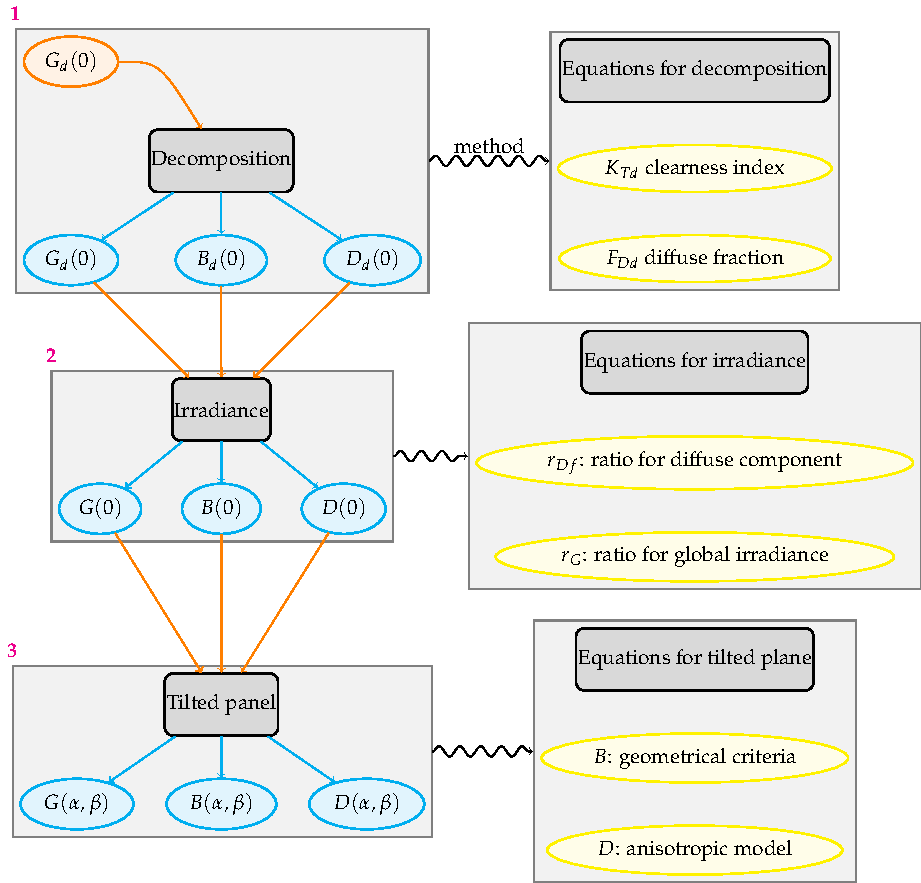
\includegraphics[width=0.6\textwidth]{figs/algorithm_outline}
  \caption{Algorithm scheme: steps on the calculation of incident irradiation at the inclined plane. Orange color means input of the calculation and blue color output or results. If a result in a previous step is used in the next one, arrows linking steps are orange. Right side of the scheme represents the method and equations needed.}
 \label{fig:algorithm_outline}
\end{figure}

\subsection{Photovoltaic energy yield}

Once the effective irradiation that reaches solar cells is being assessed, the transformation into power output depends on some factors regarding the photovoltaic system. In order to estimate  potential for photovoltaic production, the term ``yield'' is defined as the energy produced by the power installed $[\si{\kilo\watthour\per\kilo\wattpeak}]$. That energy, comes from the integration in each time step of the power output of the photovoltaic system.\\

Considering that a photovoltaic generator is composed of modules, the generator nominal power output is calculated by multiplying the power output of a single module by the number of them, assuming the same electric performance of all modules. \\

\begin{equation}\label{Pout}
P_{out}=I_{m} \cdot V_{m}
\end{equation}

\nomenclature[P_out]{$P_{out}$}{Power output from the photovoltaic module}
\nomenclature[Im]{$I_m$}{Intensity from the photovoltaic module}
\nomenclature[Vm]{$V_m$}{Voltage of a photovoltaic module}

Ambient temperature influence cells performance. The assumption used to this assessment consider a linear relationship between cell temperature and global effective irradiation, Eq.\ref{Tcelula}. NOCT in equation \ref{Tcelula} is considered constant being the temperature of a cell when it works in determined conditions: irradiance of 800 $[\si{\watt\over\metro^2}]$ and ambient temperature of $20ºC$.

\begin{equation}\label{Tcelula}
T_c=T_a + G_{ef} \cdot \frac{NOCT-20}{800}
\end{equation}

\nomenclature[T_c]{$T_c$}{Cell temperature}
\nomenclature[T_a]{$T_a$}{Ambient temperature}
\nomenclature[G_ef]{$G_{ef}$}{Global effective irradiation}

After considering all these factors, the power output of the whole system is assessed by the consideration of a common inverter for transforming DC current into AC, also arrangement losses of the generator are included. Other systems factors that influence the performance of the photovoltaic system are shadows over the generator due to the positions of the PV modules over the land. This factor is not consider in our calculations assuming that we look for an estimation of the potential yield of an area, not the product of a real PV plant. Detailed description of the software employed to the assessment, solaR, is in \cite{Lamigueiro2012}. The process for the photovoltaic output is summarized in table \ref{tabla1} including all the steps and elements involved as explained in \cite{Perpinan2009}.

\begin{table} 
  \begin{tabular}{>{\raggedright}m{6cm}>{\raggedright}m{6cm}}
    \toprule 
    Element & Method\tabularnewline
    \midrule
    PV generator & Identical modules with
    $dV_{oc}/dT_{c}=0,475\frac{\%}{\celsius}$ and $NOCT=47\celsius$. 
    The MPP point calculated as in \cite{garcia2005caracterizacion}). \tabularnewline
    \midrule
    Inverter & Efficiency equation proposed in
    \cite{jantsch1992results}:  
    \begin{equation}
      \eta_{inv}=\frac{p_{o}}{p_{o}+k_{0}^{o}+k_{1}^{o}p_{o}+k_{2}^{o}p_{o}^{2}}
    \end{equation}
    where $p_{o}=P_{ac}/P_{inv}$ is the normalized output power of the inverter. The characteristic coefficients of the
    inverters are: $k_{0}^{o}=0.01$, $k_{1}^{o}=0.025$, $k_{2}^{o}=0.05$.\tabularnewline
    \midrule
    Other losses & \begin{itemize}
    \item Average tolerance of the set of modules, $3\%$.
    \item Module parameter dispersion losses, $2\%$.
    \item Joule losses due to the wiring, $1.5\%$.
    \item Average error of the MPP algorithm of the inverter, $1\%$.
    \item Losses due to the MV transformer, $1\%$.
    \item Losses due to stops of the system, $0.5\%$.
    \end{itemize}
    \tabularnewline
    \bottomrule
  \end{tabular}
  \caption{Calculation procedure for the estimation of energy produced by a PV
    system from daily global horizontal irradiation data. Left column represents the element of the PV system and the right column the equations and methods used in each case for the efficiency of the elements.}
  \label{tabla1}
\end{table}

\nomenclature[Pinv]{$P_{inv}$}{Nominal
  power of the inverter}
\nomenclature[po]{$p_{o}$}{Normalized output power of a inverter}
\nomenclature[kinv]{$k_{i}^{o}$}{Coefficients of the
  efficiency curve of a inverter}


\section{Using Regional Climate Models}

%La cadena de modelado necesaria para obtener una estimación de la producción fotovoltaica puede incrementarse introduciendo como input una estimación o una salida de otro modelo (meteorológico, climático...) en lugar de observaciones. Este paso aumentará la incertiumbre de la potencia entregada por el sistema, pero merece la pena tomarla en consideración teniendo en cuenta la escasez de estaciones de medida que proporcionan datos de radiación.\\
The modeling chain to obtain an estimation of the photovoltaic production of a system starts with the input of the PV model. We can consider the output of an atmospheric or climate model as the input of the PV system instead of solar radiation measurements. The uncertainity of the PV power output will increase but it is worth it to consider this option because of the lack of reliable and well spread station measurements.\\  
 
%En nuestro contexto, en el cual la longitud de las series temporales es clave\footnote{el estudio climático es la evaluación del comportamiento medio de las distintas variables a lo largo del tiempo, su variabilidad y tendencias. Para poder definir una climatología se considera en consenso que son necesarios 30 años da datos.}, los modelos climáticos son una herramienta que permite evaluar el recurso presente, su evolución futura así como server de input en la cadena de modelado para estimar la potencia entregada por un sistema fotovotaico.\\  

In our context, with the purpose of analysing solar radiation and the potential PV production form a climatological point of view, climate models are a good tool that allow us to evaluate the resource in present conditions as well as its future evolution.\\

The history of climate modeling has been linked to the computational development since its beginning. The mathematical representation of the climate system was a consequence of the advance in numerical weather prediction models that took place for the first time in Princeton in 1952 and that had a fast grow. [ref and {\color{red}develop a bit more?}].\\

Climate modeling is based on a 3-D representation of the whole climatic system, where the Earth is divided  in a 3-D spatial grid whose size or resolution has evolved in time with computational power. Equations of motion, momentum and conservation laws are solved for each gridbox. As some of the atmospheric processes occurs in a finer spatial scale than the resolution of the model, parametrizations are needed for some processes such as convection. These models were first named as General Circulation Models, GCM, as their aimed was to represent main circulation flows in the atmosphere, but the development of more complex models that would start to include ocean and land, would name later these models as \textbf{Global Climate Models, GCMs}. \\

Since its origins, there has been a diversification and more research groups has developed its own climate models. Also, many international framework initiatives has unify efforts to understand better the future evolution of climate with the intensification and promotion of research collaboration programs that include all the models (WCRP, IPCC, CLIVAR...)\\   
%``L. F. RichardsonZ was the first to promote the idea that future weather could be predicted by numerically integrating the equations of fluid motion using the present weather as the initial condition.  The first successful numerical forecasts used a  set of equations that are greatly simplified compared to Richardson’s and for which the solution is less sensitive to the initial conditions.''

Global climate models provides reliable information about the possible evolution of climate in large scales. Their horizontal resolution, however, covers areas with very different regional characteristics, which potentially miss some information that affect in a particular manner to smaller and vulnerable areas.\\

It was in the early 90s (Dickinson 1989 and Giorgi 1990) when it was proposed to use global models as the necessary boundary conditions to force a 'limited area model LAM'. Those LAMs had been used for numerical weather prediction forecast, but they were applied to predict the weather just few days in advance. The idea of run these simultaions for longer periods will result in the evolution of \textbf{Regional Climate Modeling}, what would provide regional climate information of processes that occurs in a spatial scale not resolved by a global models.\\

In a similar way than the GCMs, RCMs community has expanded in last decades and the number of research groups has increased. Also, some international initiatives try to engage different groups and modellers to develop better models and simulations (PRUDENCE, ENSEMBLES,CORDEX, EURO-CORDEX, MED-CORDEX).\\

In the present work we make use of RCMs focused on the Mediterranean area, considering the models and simulations included in the EURO-CORDEX and MED-CORDEX projects.\\

These RCMs can provide the necessary atmospheric variables for the analysis of renewable energy resources. Due to its complexity and the need of parametrizations for some atmospheric processes, they can have sistematic bias that make difficult to use them for resource assessment. However, due to the low frequency variability observed in some variables and to the importance of considering the future projections, they are a valuable tool for analysing renewable energy resources and its evolution. Besides, the use of climate models allows to study specific climatic events and to understand its mechanisms, linking the implications of those situations with renewable generation.\\

For chapter 6, ``Impact of aerosols in photovoltaic energy production'', only one RCMs is used. Three different simulations are used in this chapter in order to quantify the sensitivity of PV energy production to changes in atmospheric aerosols content. The simulations are centered in the Mediterranean area, with the domain described by the MED-CORDEX initiative. The simulations length and characteristics of the aerosols dataset included are explained in detailed in the corresponding chapter.\\


% \begin{figure}
%   \centering
%   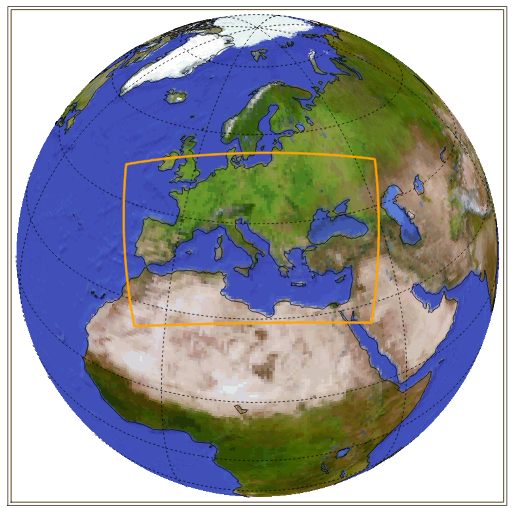
\includegraphics[width=0.4\textwidth]{DataMethodsFIGS/medcordex2}
%   \caption{Med-CORDEX domain}
%  \label{fig:medcordex}
% \end{figure}

\section{Future projections and scenarios}

Behind the comprehensive study of the climate system it is not only the interest of a deeper understanding of the physics processes but also there is a concern about the impact that a changing climatic system could have in the ecosystems and different species of the Earth.\\ 

The Intergovernmental Panel on Climate Change, IPCC, was launched in 1992 and it is an international organism that was founded by the World Meteorological Asociation, WMO, and the United Nations Environmental Program, UNEP. Its purpose was to gather together all the scientific information available about the anthropogenic climate change. This information will summarize our knowdlege about climate change, its impacts as well as some mitigation strategies were elaborated.\\

In order to elaborate the climate scenarios, which means the possible evolution of the climate system based on the actual climate conditions and models, it is necessary also to generate different plaussible scenarios of emissions. The development of these emission scenarios of greenhouse gases or aerosols will be based on the assumptions about technological changes or demographic criterias as well as the socioeconomic development of each region. Those scenarios, with different options for the future evolution, will be the driving force for the climate simulations in order to elaborate the climate projections.\\

The first emission scenarios were elaborated in the 90s and they have changed since then. For the 5th AR of the IPCC, that was released 2014 were defined the RCP scenarios. They are different 'representative concentrations pathaways' that correspond to the one of the possible scenarios that leads to an specific radiative forcing, i.e, the RCP8.5 represents a radiative forcing of 8.5 $[\si{\watt\per\metro^2}]$\\

For chapter 7, ``Future projections for PV technology'', several RCMs and its correspondin GCMs are used. The simulations include the historical period and the future scenario RCP8.5 or RCP4.5. The analysis of the results will be done with respect to a reference historical period.\\

In table \ref{climatemodels} there is a summary of the climate models and the simulations that are used in chapter 6 and 7.\\

\begin{table}[h!]
  \begin{tabular}{c|>{\raggedrigth}m{1.2cm}>{\raggedright}m{1.5cm}>{\raggedright}m{2cm}>{\raggedright}m{1.5cm}>{\raggedright}m{1.5cm}>{\raggedright}m{2cm}}
    \toprule 
    Study & \centering{Climate Model}  & &  \tabularnewline
    \midrule                                                         
    & \centering{GCM} & \centering{RCM} & \centering{Domain} & \centering{Resolution RCM} &\centering{Simulation} \tabularnewline                                            
    \midrule
     Aerosols' impact & \centering{CNRM-CM5} & \centering{CNRM-ALADIN53} & \centering{MED-CORDEX} & \centering{44º} & \centering{AER}\midrule\\
    \centering{NO-AER}\midrule\\
    \centering{TREND}
    \tabularnewline
   \midrule
    Future projections & \centering{CNRM-CM5} & \centering{ALADIN53}\midrule\\
    \centering{RCA4}\midrule\\
    \centering{CCLM4}\midrule & \centering{EURO-CORDEX} & \centering{11º} & \centering{HIST/RCP85}\\
    \centering{HIST/RCP85}\\
    \centering{HIST/RCP85}
    \tabularnewline
          & \centering{ICHEC-EC-EARTH} & \centering{RACMO}\midrule\\
    \centering{RCA4}\midrule\\
    \centering{CCLM4}\midrule & \centering{EURO-CORDEX} & \centering{11º} & \centering{HIST/RCP85}\\
    \centering{HIST/RCP85}\\
    \centering{HIST/RCP85}
    \tabularnewline
 \bottomrule
  \end{tabular}
  \caption{Summarize of the climate models (global, GCM, or regional, RCM) used in chapters 7 and 8. The name of the global model includes the institute that elaborate the simulation and afterwards the global models's name. The domain of the simulations is MED-CORDEX or EURO-CORDEX, described in the referenced paper.}
  \label{climatemodels}
\end{table}


% * Los modelos climáticos proporcionan las variables atmosféricas necesarias para el análisis del recurso de energías renovables. Debido a su complejidad y la necesidad de parametrizar ciertos procesos, pueden contener sesgos importantes que dificulten su utilización como modelos para evaluación de recurso. Sin embargo, debido tanto a la variabilidad de baja frecuencia observada en muchas variables del sistema (global dimmimg and brigthenning) como a la importancia de considerar las distintas proyecciones de cambio climático, se han convertido en una herramienta importante para considerar la evolución de los recursos. Además, su uso permite estudiar eventos climáticos concretos y entender sus mecanismos, permitiendo estudiar las implicaciones de esas situaciones en la generación renovable.\\


%The first idea of modeling the climatic system came from ..
%The climate system is modeled by Global Climate Models, GCMs, that represents the climate system in a 3-dimensional way.
%``Global climate models are three‐dimensional representations of the climate system and its components. Using mathematical equations, climate models can simulate the exchange of air, water, and energy between components, given user‐specified input parameters. Using model validation techniques and sensitivity studies, climate modelers can assess a model's accuracy in simulating global climate change as well as establish a cause‐and‐effect relationship between various climate drivers and observed changes. Projections of future global climate change can be obtained by specifying different scenarios of future greenhouse gas emissions. Output from global climate models can take the form of a time series of global change in a particular climate variable (such as temperature), or of a global map depicting the spatial pattern of change in that variable at a future point in time. A great deal of uncertainty is associated with climate modeling, stemming from unknown future emissions, intermodel uncertainty, and uncertainty about various climate processes.''


%El sistema climático y su modelización. Modelos de circulación globales. Orígenes de los modelos de área limitada, LAM. Downscalling dinámico que pasó a ser el desarrollo de los RCM.



